\documentclass{ltjsarticle}

\usepackage{amsmath}
\usepackage{amssymb}
\usepackage{amsthm}
\usepackage{ mathrsfs }
\usepackage{enumerate}
\usepackage{bbm}
\usepackage{lipsum}
\usepackage{fancyhdr}
\usepackage{tikz-cd} 
\usetikzlibrary{graphs}
\usepackage{luatexja-ruby} 
\usepackage{graphicx} 
\graphicspath{ {./../../images/} }

\newtheorem{theorem}{定理}[section] 
\newtheorem{proposition}{Proposition}[section] 
\newtheorem{definition}{定義}[section] 
\newtheorem{problem}{問題}
\newtheorem{postulate}{公準}[section] 
\newtheorem{lemma}{Lemma}[section] 
\newtheorem{notation}{Notation}[section] 
\newtheorem{remark}{注釈}[section] 
\newtheorem{corollary}{系}[section] 
\newtheorem{terminology}{Terminology}[section] 
\newtheorem{example}{例}[section] 
\newtheorem{step}{手順} 
\newtheorem{solution}{解答}[section] 
\newtheorem{fact}{事実}[section] 

\DeclareMathOperator{\diam}{diam}
\DeclareMathOperator{\Gal}{Gal}
\DeclareMathOperator{\rank}{rank}
\DeclareMathOperator{\Hom}{Hom}
\DeclareMathOperator{\Dom}{Dom}
\DeclareMathOperator{\Ann}{Ann}
\DeclareMathOperator{\grad}{grad}
\DeclareMathOperator{\Span}{Span}
\DeclareMathOperator{\interior}{int}
\DeclareMathOperator{\ind}{ind}
\DeclareMathOperator{\supp}{supp}
\DeclareMathOperator{\ob}{ob}
\DeclareMathOperator{\Spec}{Spec}
\DeclareMathOperator{\MaxSpec}{MaxSpec}
\DeclareMathOperator{\PreSh}{PreSh}
\DeclareMathOperator{\Sh}{Sh}
\DeclareMathOperator{\Fun}{Fun}
\DeclareMathOperator{\Ext}{Ext}
\DeclareMathOperator{\Aut}{Aut}
\DeclareMathOperator{\Ker}{Ker}
\DeclareMathOperator{\Image}{Im}
\DeclareMathOperator{\Coker}{Coker}
\DeclareMathOperator{\id}{id}
\DeclareMathOperator{\Mod}{Mod}
\DeclareMathOperator{\QCoh}{QCoh}
\DeclareMathOperator{\Coh}{Coh}
%\newcommand*{\name}[\num_arguments][default values]{{\color{#1}\Large #2}}
\newcommand*{\Z}{\mathbb{Z}}
\newcommand*{\Q}{\mathbb{Q}}
\newcommand*{\R}{\mathbb{R}}
\newcommand*{\multivar}[2]{{#1_1,\cdots,#1_{#2}}}
\newcommand*{\localization}[2]{#1_{\mathfrak{#2}}}
\newcommand*{\ringedspacemorph}[1]{(#1,#1^{\#})}
\newcommand*{\sheaf}[2]{(#1,{\mathcal{#2}}_{#1})}
\newcommand{\fib}[1]{%
  \mathbin{\mathop{\times}\limits_{#1}}%
}
\newcommand{\tens}[1]{%
  \mathbin{\mathop{\otimes}\displaylimits_{#1}}%
}
\title{授業ノート}
\author{ボン補習校高校数学}
\date{6月6日}

\begin{document}

\maketitle

\section{順列と組み合わせ}

$A,B,C,D,E$の五人から三人選んで並べる並べ方は
\begin{equation*}
5\times 4\times 3 =60\text{通り}
\end{equation*}
あることを覚えていますか。これは、最初の一人を選ぶ選び方は５通り、その後に次の人を選ぶ選び方は４通り、のように考えるとわかると思います。では五人のうちから三人選ぶ選び方はいくつあるでしょうか。ここで次の並べ方を比べてみます。
\begin{equation*}
ABC, ACB,BAC,BCA,CAB,CBA
\end{equation*}
並べ方は違いますが、三人の選び方は全て同じです。ほかの選び方、例えば$A,B,D$を選んだ時も同じようにダブりが出てしまいます。ここで注目したいのは、ダブりの数は選び方に関係なく常に同じだということです。たとえば、
\begin{equation*}
ABC,ADB,BAD,BDA,DAB,DBA
\end{equation*}
のように六つダブりが出てきます。なぜなら、このダブりの数は選んだ三つを並べ方の数と一致するからです。このばあい、$3\times2\times1=6$通りのダブり方があります。このよう選んだ人が同じになるようにグループ分けすると、そのようなグループは
\begin{equation*}
60\div 6 = 10\text{グループ}
\end{equation*}
あることになります。よって五人の中から三人を選ぶ選び方は１０通りあります。このことを一般化してみましょう。

\begin{theorem}
$n$この中から$k$こを選ぶ選び方は
\begin{equation*}
{n\choose k} = {\frac {n(n-1)\cdots (n-k+2)(n-k+1)} {k(k-1)\cdots 2\cdot 1}}
\end{equation*}
\end{theorem}



次の定理を考えてみましょう。

\begin{align*}
(x+y)^n &= \sum_{k=0}^n {n\choose k}x^ky^{n-k},\\
&  =  {n\choose 0}x^0y^{n}+{n\choose 1}x^1y^{n-1}+{n\choose 2}x^2y^{n-2}+\cdots+{n\choose n-1}x^{n-1}y^{1}+{n\choose n}x^ny^{0}.
\end{align*}

これは
\begin{align*}
(x+y)^n=(x+y)\cdots(x+y)
\end{align*}
と書けることにより、$x^ky^{n-k}$を作ることは$n$このカッコから$x$を選ぶカッコを$k$こ選ぶことと同じなので上の士気が得られます。

\begin{problem}
\begin{equation*}
\sum_{k=0}^n {n\choose k} = 2^n.
\end{equation*}
\end{problem}
\begin{proof}[解答]$\:$
\par 上の定理で$x=y=1$を代入。
\end{proof}

\section{確率分布}

\begin{theorem}
二つの現象がおこる確率をそれぞれ$a,b$とする。もし、それらの現象がお互いに影響しないなら、二つの現象がどちらも起こる確率は$ab$となる。
\end{theorem}

\begin{example}
コインを2枚投げて両方表となる確率は${\frac 1 2}\times{\frac 1 2} = {\frac 1 4}$である。
\end{example}

\begin{definition}
勝つ確率が$p$の勝負を考える。$n$回のこの勝負をして$k$回勝つ確率は
\begin{equation*}
{n\choose k}p^k(1-p)^{n-k}
\end{equation*}
で計算される。
\end{definition}


\section{宿題}
\par\textbf{1.モンティ・ホール問題}\\
三つの扉があります。あなたは扉を選んで、選んだ扉の向こうにあるものもらうことができます。扉の一つには高級車が、二つには山羊が入っています。高級車が入っている扉が選ばれる確率は一様分布になるとする。今、あなたは一つ扉を選びました。ここでゲームマスターはあなたが選ばなかった扉の中から山羊が入っているものを一つ選んで開けます。残った扉は２つです。
\par ゲームマスターがヤギの入っている扉を開けた後、あなたはもう一度自分で開ける扉を選ぶことができます。選んだ扉を変えるのと変えないのではどちらの方が高級車がもらえる確率が上がるでしょうか。（ヒント：もし扉の数が１００個でそのうち９９個には山羊が入っているとする。ここで、あなたが扉を選んだ後、ゲームマスターは残りの９９個の扉のうち９８個山羊が入っているものを開けます。このときあなたは選んだ扉を変えますか変えませんか）
\par\textbf{2.偽陽性のパラドックス}\\
ウイルスの検査は必ずしも100％正しいとは限りません。たとえばコロナウイルスの検査では次の四つのケースがあります。
\begin{enumerate}
\item \ltjruby{\textbf{真陽性}}{しんようせい}：実際にコロナにかかっていて、検査でコロナにかかっているとでる。
\item \ltjruby{\textbf{真陰性}}{しんいんせい}：コロナにかかっておらず、検査でもかかっていないとでる。
\item \ltjruby{\textbf{偽陽性}}{ぎようせい}：コロナにかかっていないのに、検査でコロナにかかっているとでる。
\item \ltjruby{\textbf{偽陰性}}{ぎいんせい}：コロナにかかっているのに、検査でもかかっていないとでる。
\end{enumerate}
ここでコロナの\ltjruby{罹患率}{りかんりつ}（百人中何人コロナにかかっているかの割合）が$0.1\%$（つまに、千人に一人コロナに感染している）とします。また検査の精度（コロナにかかった人百人中検査で陽性となる人の割合）はおよそ$99\%$、また特異度（かかっていない人がかかっていないと検査される割合）も$99\%$とする。ここで、あなたは検査でコロナ陽性と出ました。あなたが実際にコロナにかかっている確率はどのくらいでしょうか。100万人を検査した時のことを考えてみましょう。
\begin{enumerate}[ステップ1.]
\item 100万人のうち実際にコロナにかかっているのは何人でしょうか。
\item 実際にコロナにかかっている人のうちで、検査で陽性となるのは何人でしょうか。
\item コロナにかかっていないのに検査で陽性となる人は何人いるでしょうか。
\item 検査で陽性と診断されるひとは全部で何人いるでしょうか。
\item 検査で陽性と診断されたうち何％が実際にコロナにかかっているでしょうか。
\end{enumerate}
\par\textbf{3.二項分布}\\
ある勝負をして勝つ確率を$p$負ける確率を$1-p$とする。この時$n$回やって$k$回勝つ確率は
\begin{equation*}
{n\choose k}p^k(1-p)^{n-k}
\end{equation*}
で表される。なぜこの公式で計算できるのかを考えてみよう。（ヒント：$k$個のどんな勝負を選んでいますか）。
\par サイコロを投げると$1~6$それぞれの目が出る確率は${\frac 1 6}$でそれ以外の目が出ることはありません。これらが起こりうるすべてのことがらなので全部足すと
\begin{equation*}
{\frac 1 6}+\cdots+{\frac 16} = 1
\end{equation*}
となります。ここでこの二項分布の時を考えてみましょう。起こりうる事柄は$n$回の勝負のうち$0,1,2,3,\cdots,n-1,n$回かつ事。これらの確率を全て足すと$1$になることを示してみよう。（ヒント
\begin{equation*}
(x+y)^n = \sum_{k=0}^n{n\choose k}x^ky^{n-k}
\end{equation*}
を使おう。ここで$x,y$に入るのはどんな数かな。）
\par\textbf{4.サイコロの確率}\\
サイコロを$n$回ふって$k$回３の倍数の目が出る確率はいくつですか。
\begin{enumerate}
\item サイコロを振って三の倍数の目が出る確率は幾つでしょうか。
\item ステップ１を使ってこの場合の二項分布を考えてみよう。
\end{enumerate}
\par\textbf{5.パスカルの三角形}
\begin{equation*}
{4 \choose 0},{4\choose 1},{4\choose 2},{4\choose 3},{4\choose 4}
\end{equation*}
を全て計算してみよう。
\begin{center}
\begin{figure}[h]
	\centering
    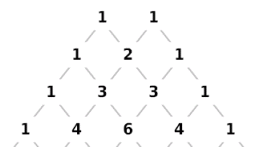
\includegraphics[scale=0.5]{pascal_triangle}
    \label{fig:Euler_1}
\end{figure}
\end{center}
パスカルの三角形とは上のように、自分の上にある数字二つを足した数が自分と同じになるような三角形です。例えば3段目の真ん中では$1+2=3,2+1=3$となっているのがわかると思います。ここで、先に計算した${4\choose k}$と4段目を比べてみよう。この三角形を使って${5 \choose k}$を予想してみよう。
\end{document}